%\section{Conclusiones}
%\subsection{Sobre la gesti\'on}
\begin{frame}
	\frametitle{Conclusiones}
	\framesubtitle{Sobre la gesti\'on}
	
	\begin{columns}[T] % contents are top vertically aligned
		
		\begin{column}[T]{0.35\linewidth} % each column can also be its own 
			%environment
			\begin{itemize}
				\item Pese a las metodolog\'ias \'agiles ha habido retraso
			\end{itemize}
		\end{column}
		
		\begin{column}[T]{0.65\linewidth} % alternative top-align that's better 
			%for graphics
			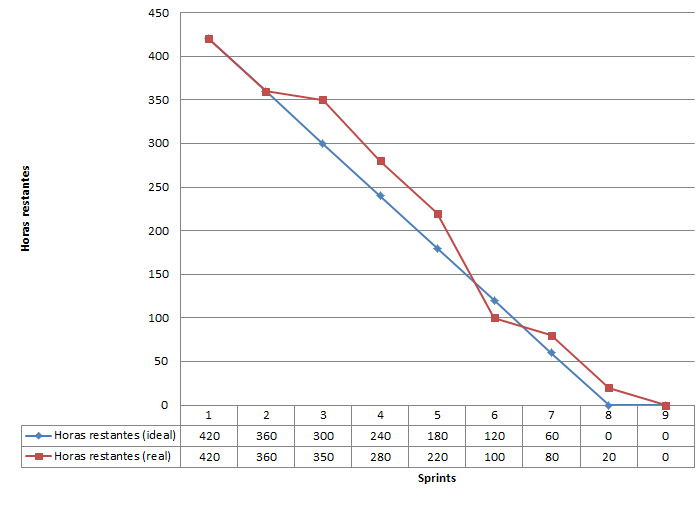
\includegraphics[width=1.0\linewidth]{./Figures/burndown.png}
		\end{column}
	\end{columns}
\end{frame}

%\subsection{Riesgos que se han cumplido}
\begin{frame}
	\frametitle{Conclusiones}
	\framesubtitle{Riesgos que se han cumplido}
	\begin{itemize}
		\item Tener que cambiar de biblioteca
		\item Nuevos requisitos
		\begin{itemize}
			\item Seleccionar el momento de inicio de sincronizaci\'on del 
			v\'ideo
			\item En un mismo XML poder a\~nadir m\'as de un intervalo
			\item Visualizar un \'arbol lateral con las propiedades y 
			observaciones
		\end{itemize}
	\end{itemize}
\end{frame}

%\subsection{Personales}
\begin{frame}
	\frametitle{Conclusiones}
	\framesubtitle{Personales}
	
	\begin{itemize}
		\item S\'indrome del programador
		\item Dif\'icil programar sin documentaci\'on
		\item Estar fuera de la zona de ``confort"
	\end{itemize}
\end{frame}

